\chapter{Muon Lifetime}

\section{Introduction}

In this lab, you will analyze data to cacluate the muon lifetime.
This lab has only Jupyter notebook entries.

\begin{figure}[htbp]
\begin{center}
{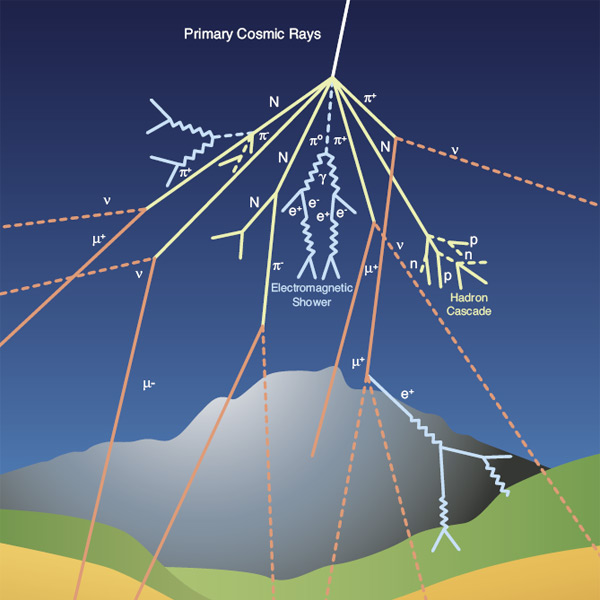
\includegraphics[width=0.35\textwidth]{figs/labs/muon/cosmic_ray.jpg}}\\
\end{center}
\caption{\label{fig:cosmic}  Cosmic ray shower induced by a primary cosmic ray (typically protons) striking an atom in the upper atmosphere.}\end{figure}

The muon is a fundamental particle in the Standard Model of particle
physics.  It is essentially a heavier version of the electron.  Like
the electron, the muon has a corresponding anti-particle, the
anti-muon ($\mu^+$).  Muons are readily available for study because
they are produced as a result of showers that are induced by incident
cosmic rays that constantly bombard the earth.  Typical primary cosmic
rays are protons, and there collisions with nuclei in the upper
atmosphere produce mainly protons, neutrons, and pions.  The
subsequent decays of these particles produce electrons, neutrinos, and
the muons we will be studying.  The flux of muons at sea-level is
about 1 per ${\rm cm}^2$ per minute, and this population has a mean
kinetic energy of about $4~\rm GeV$.  Such muons are highly
penetrating: they pass quite readily through buildings.

The muon decays via the weak interaction, its most probable decays being:
\begin{eqnarray*}
\mu^- \to e^- + \bar{\nu}_e \nu_\mu,\\
\mu^+ \to e^+ + \bar{\nu}_\mu \nu_e.
\end{eqnarray*}
As fundamental particles, muons are indistinguishable from one
another, and therefore the decay rate for a population of $N$ muons
must be simply proportional to $N$:
\begin{displaymath}
\frac{dN}{dt} = -\frac{N}{\tau}
\end{displaymath}
The solution to this differential equation is:
\begin{displaymath}
N(t) = N(0) \exp(-t/\tau).
\end{displaymath}
The muon lifetime has the value 
\begin{displaymath}
\tau_\mu = 2.1969811(22) \mu s
\end{displaymath}
in vacuum as reported by the Particle Data Group (PDG) with the
uncertainty in parenthesis.  Interactions with the scintillator
material in this experiment lead to a slightly different expectation
for the lifetime as discussed below.

Muons are produced at a typical height $15~\rm km$ above sea-level,
and so, in the earth frame, their transit time from the upper
atmosphere to our lab is therefore about $50~\rm \mu s$ or about 20
lifetimes.  The fact that we see an appreciable number of them at sea
level, given an upper limit on their production rate in the
atmosphere, is clear evidence for the time dilation effects of special
relativity.

\section{Experimental Setup}

\begin{figure}[htbp]
\begin{center}
{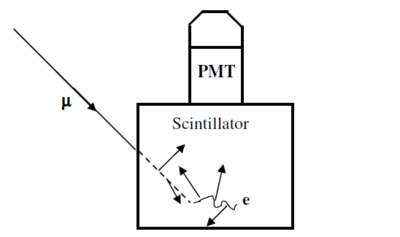
\includegraphics[width=0.55\textwidth]{figs/labs/muon/setup.png}}\\
\end{center}
\caption{\label{fig:setup}  Experimental setup.}\end{figure}

The active component of the particle detector used in this experiment
is a polyvinyltoluene-based plastic scintillator in the shape of a
cylinder with a $15~\rm cm$ diameter and a $12.5~\rm cm$ height.  All
materials absorb energy due to the passage of ionizing radiation.
Scintillators are materials which re-emit a fraction of this energy as
visible light, typically in the blue to near UV range.  The light
yield is relatively low, so a sensitive photomultiplier tube is used
to amplify a modest number of photons into a large easily measurable
voltage.

\begin{figure}[htbp]
\begin{center}
{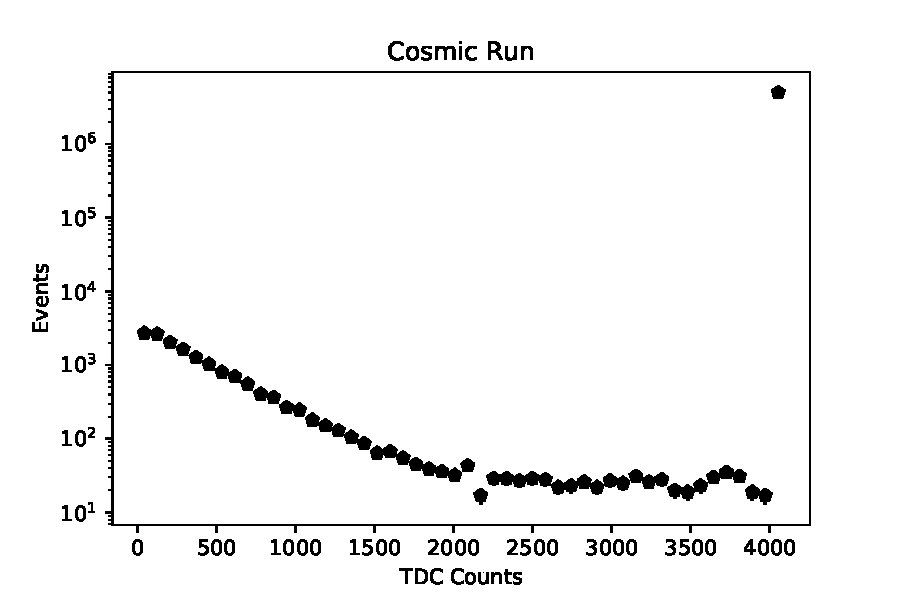
\includegraphics[width=0.65\textwidth]{figs/labs/muon/cosmics_raw.pdf}}\\
\end{center}
\caption{\label{fig:cosmics_raw}  Three days of cosmic ray data, plotted as the distribution in digitized time measurement (TDC counts).}
\end{figure}


Muons are therefore constantly passing through the scintillator,
depositing energy, and causing observable PMT pulses which are
recorded by the data acquisition system (DAQ).  Occasionally, however,
a relatively low-energy muon enters the scintillator and deposits all
of it's kinetic energy, coming to rest.  As an unstable particle, it
eventually decays into a highly-energetic electron and neutrinos.  The
electron deposits additional energy in the scintillator which is
observed as a second pulse.  The time interval between two consecutive
pulses is digitized using a time-to-digital (TDC) converter, which
converts analog time interval into a digital number.  In this case, we
use a 12-bit TDC, so the measured digital values are integers in the
range from 0 to $2^{12}-1 = 4095$.  To interpret these raw TDC counts
as a time value in microseconds, you will need to calibrate the TDC as
described below.

Three days of data has already been collected for you, and is plotted
in Fig.~\ref{fig:cosmics_raw} .  This data is available on the course
web site in the file {\tt cosmics.npy} available You load this data
using the numpy {\tt load} command, taking care to handle the
directory path correctly.  As can be seen from the plot, most of the
recorded events have the maximum possible value 4095.  This is how the
DAQ records a single pulse, with no secondary pulse in the timing
window of the TDC.  This is what happens most of the time.

The remaining events, with a measured time below the maximum value, are from events were two pulses were detected within the timing window of the TDC.  This time
interval, the decay time of the muons in this population, will have a
time-dependence given by:
\begin{displaymath}
-\frac{dN}{dt} = \frac{N(0)}{\tau} \exp(-t/\tau)
\end{displaymath}
which you will use to extract the muon life time.  This is possible because the muon decay rate ($\lambda$)
and it's lifetime $\tau$ are simply recipocrals:
\begin{displaymath}
\lambda \equiv \frac{-\frac{dN}{dT}}{N(t)} = \frac{1}{\tau}.
\end{displaymath}
This exponential decay feature is clearly visible in the raw data as the downward sloping line on the right side of this semilog plot.

There is an additional source of background for two pulse events, which arises from the possibility for two muons to arrive independently within the time window of the TDC.   Sine the arrival time of the two muons is independent, this contribution is flat in time, and is clearly visible in the raw data on the left-hand side, where the exponential contribution becomes small.

\section{Calibration}

\begin{figure}[htbp]
\begin{center}
{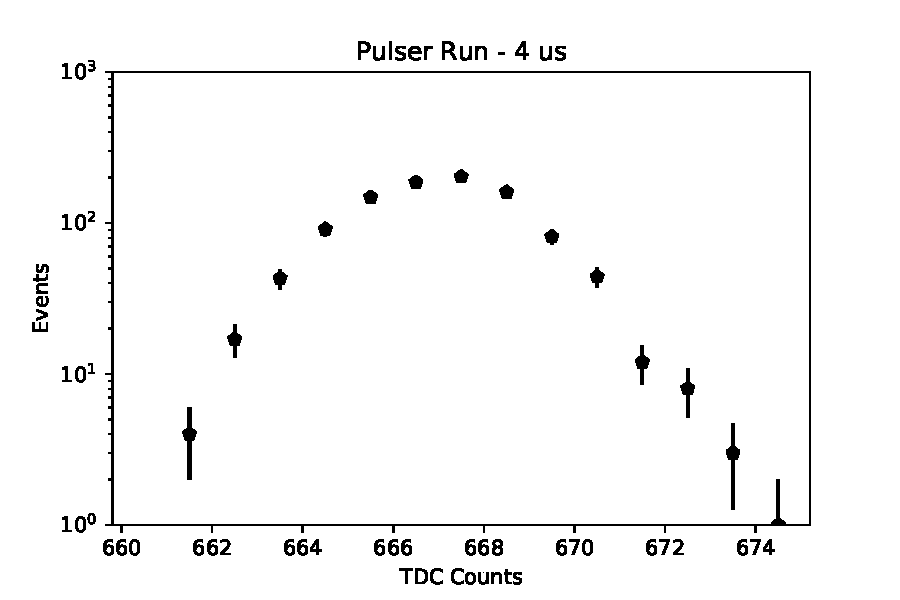
\includegraphics[width=0.65\textwidth]{figs/labs/muon/pulser_4_raw.pdf}}\\
\end{center}
\caption{\label{fig:pulser_raw}  Calibration run with pulses spaced $4~\mu s$ apart.}
\end{figure}

To interpret the output of the TDC (digital TDC counts as integers in
the range from 0 to 4095) as physical times in units of microseconds,
a calibration is needed.  We are using a good TDC which we can assume has a linear response, meaning that the time interval and TDC counts are related as:
\begin{displaymath}
TDC = a \cdot \Delta t  + b 
\end{displaymath}

To determine the calibration parameters $a$ and $b$ we use an LED
pulser feature built into the detector.  The LED pulser feature
flashes light into the PMT in a controlled manner, so that two pulses
a distance $\delta t$ in time apart are sent repeatedly to the TDC.
An example of 1000 pulser events with $\Delta t = 4 \mu s$ is shown in
Fig.~\ref{fig:pulser_raw}.  A total of four pulser runs of 1000 events
each with $\Delta t = 1,2,4,8$ have already been collected.  The data
from these four calibration runs available on the course website with
names like {\tt pulser{\_}4.npy} for the $\Delta t = 4~\rm \mu s$ run.

\begin{plot}
or each pulser run, compute the mean value of the recorded data and an uncertainty on this mean value.
Plot these mean values, and their uncertainties, versus $\Delta t$.  Fit the linear response to obtain the parameters $a$ and $b$.  Plot the best fit linear function alongside the data.
\end{plot}

\section{Muon Lifetime Analysis}

The calibration constants $a$ and $b$ are used to convert the TDC
counts of the recorded comsic ray data into physical time intervals.

\begin{plot}
Using your calibration contants, convert your comsic data TCD counts
into time intervals, and plot the ditribution as a histogram.  You
should omit all events with RAW TDC count of 4095, as these are single
pulse events.  Fit the distribution to an exponential function plus a
constant value for the flat (combinatoric) background.  Plot your fit
function against the recorded data.  Report the statistical
uncertainty on the fitted value for the muon lifetime.  In addition,
there are several systematic uncertainties associated with the
experiment.  The largest is the effect of material interactions on the
lifetime of the muon, which is about $5\%$.  Other systematic effects
are smaller, and can be neglected.
\end{plot}

%\section{Muon / Anti-Muon Ratio}

%Due to additional decay processes when captured by an atomic nucleus, the decay time of the negatively %charged muon in matter is lower than its free space value:
%\begin{eqnarray*}
%\tau_- &=& 2.043(3) \times 10^{-6} \mu s \\
%\tau_+ &=& 2.1969811(22) \times 10^{-6} \mu s
%\end{eqnarray*}
%where we have used the measured values in carbon, which should be close to value for our organic %scintillator.

%As discussed in class, you can determine the ratio $\rho$ of anti-muons to muons from the relation:
%\begin{displaymath}
%\rho = - \frac{\tau_+}{\tau_-} \cdot \frac{\tau_- - \tau}{\tau_+ - \tau}
%\end{displaymath}
%where $\tau$ is the measured valued of the muon lifetime.


